\documentclass{article}

%Headers
\usepackage[dvips]{graphicx}    %package that does pdfs
\usepackage{color}              %this needs to be here also

\title{Simple Document Example}
\author{Christopher W. Lum\thanks{Research Assistant Professor, William E. Boeing Department of Aeronautics and Astronautics, University of Washington; Guggenheim Hall Room 211, Box 352400, Seattle, WA 98195-2400.  Email: lum@uw.edu}}
\date{September 16, 2018}

\begin{document}
\maketitle

\begin{abstract}
This is a simple example showing how to generate a document using LaTeX.  This is designed to illustrate several constructs in LaTeX such as sections, figures, equations, tables, creating a bibliography, etc.
\end{abstract}

%Note that the '*' surpresses the section numbering
\section*{Nomenclature}
\label{sec:nomenclature}
\begin{tabbing}
    XXXXXXXX \= \kill% this line sets tab stop
	GCS					\> Ground Control System\\    
	UA/UAS              \> Unmanned Aircraft/Unmanned Aerial System\\
	UW					\> University of Washington	
\end{tabbing}

\section{Experimental Methodology}
This section describes the experimental methodology.

\subsection{Aircraft}
The goals of this experiment are as follows:

%Illustrate using a list
\begin{itemize}
    \item Flight test a small unmanned aerial system (UAS).
    \item Demonstrate viability of using an aviation tranponder onboard a UAS.
\end{itemize}

The aircraft used in the experiment is shown in Figure~\ref{fig:Aircraft}.  This was flight tested on several occasions \cite{Lum_ADSB_sUAS_2017} and uses autonomous algorithms to perform search and rescue \cite{Lum_Searching_JACIC_2010}.  

%Illustrate inserting a figure
\begin{figure}[ht]
	\centering
    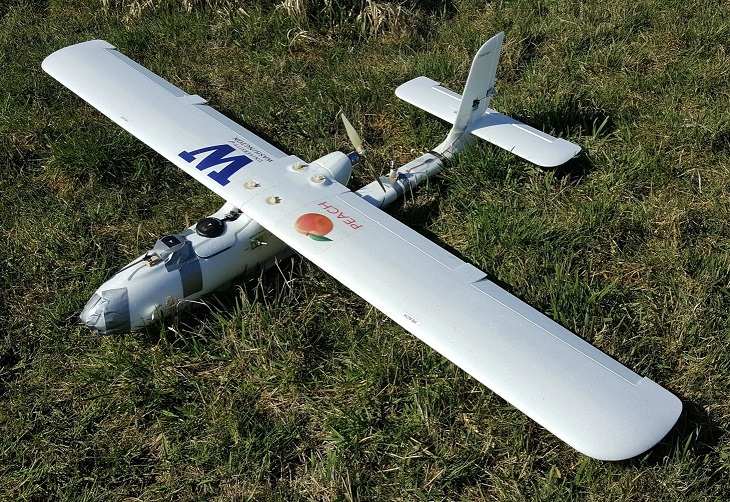
\includegraphics[width=3in]{Aircraft}
    \caption{Aircraft flown in the experiment.}
    \label{fig:Aircraft}
\end{figure}

Characteristics of the aircraft are shown in Table~\ref{table:UASPerformance}.

%Illustrate inserting a table
\begin{table}
	\begin{center}
	\begin{tabular}{|p{6cm}|p{6cm}|}
	\hline
	\textbf{Aircraft Characteristics} & \textbf{Values} \\
	\hline
	Total Weight & 2.917 kg \\
	\hline
	Endurance & $\approx$ 15 minutes \\
	\hline
	Center of Gravity & 17.75 in. aft of aircraft nose\\
	\hline
	\end{tabular}
	\caption{UAS performance specifications.}
	\label{table:UASPerformance}
	\end{center}
\end{table}

The ground control station (GCS) is shown in Figure~\ref{fig:GroundControlStation}.  

\begin{figure}[ht]
	\centering
    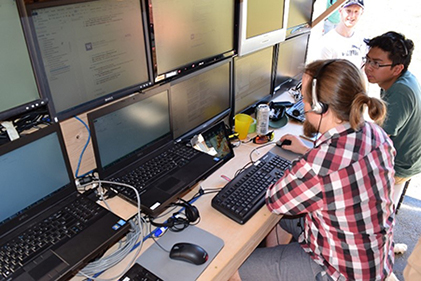
\includegraphics[width=3in]{GroundControlStation}
    \caption{Operators at the GCS.}
    \label{fig:GroundControlStation}
\end{figure}

\subsection{Algorithms}

An example of an equation is given in Eq.~\ref{eqn:KalmanUpdate}.

%Illustrate inserting an equation
\begin{equation}
	K = P_{predicted} H^{T} \Big( H P_{predicted} H^{T}+R\Big) ^{-1}
	\label{eqn:KalmanUpdate}
\end{equation}

%Illustrate breaking the document into several .tex files and then including them together with 'input'
\section{Conclusions}
Here are the conclusions.  Note that this is a separate .tex file which is included into the larger document.

%Illustrate creating a bibliography by referring to an external bibliography file (SampleBibliography.bib).  Note that you must chose a style to determine how the bibliography is presented
\bibliography{SampleBibliography}
\bibliographystyle{aiaa}

\end{document}
